Bouajjani and Emmi created a formal model of isolated hierarchical parallel computation that covers many existing task parallel languages (e.g., Cilk, X10, Chapel, Habanero, etc.) \cite{bouajjani}. Real world task parallel models are not isolated so tasks may share memory (intentionally or otherwise). This paper uses the formalism of Bouajjani and Emmi to define the construction of the computation graph from program execution but adds global variables. As before, a \emph{region} groups tasks by storing task handles, but now each region also holds a variable that can be shared. Tasks are expanded to include access lists to denote region variables available for reading or writing.  

\section{Surface Syntax}

\begin{figure}
  \begin{center}
\[
  \begin{array}{rcl}
\textbf{P} &::=& (\textbf{proc}~p~(\textbf{var}\ \texttt{l} : L)~s)* \\
\textbf{s} &::=& s;~s \alt \texttt{l} := e \alt \texttt{l}(r)\ := e \\
&\alt& \textbf{skip} \alt  \textbf{assume}~e \\
&\alt& \textbf{if}~e~\textbf{then}~s~\textbf{else}~s \alt \textbf{while}~e~\textbf{do}~s \\
&\alt& \textbf{call}~\texttt{l}\ := p~e~\vec{r_\delta}~\vec{r_\omega} \alt \textbf{return}~e \\
&\alt& \textbf{post}~r \leftarrow p~e~\vec{r}~\vec{r_\delta}~\vec{r_\omega}~d \\
&\alt& \textbf{await}~r \alt \textbf{ewait}~r \\
  \end{array}
\]
  \end{center}
  \caption{The surface syntax for task parallel programs.}
  \label{fig:syntax}
\end{figure}

The surface syntax for the language is given in \figref{fig:syntax}. A program \textbf{P} is a sequence of procedures. The procedure name $p$ is taken from a finite set of names \texttt{Proc}. Each procedure has a single $L$-type parameter \texttt{l} taken from a finite set of parameter names \texttt{Vars}. The body of the procedure is inductively defined by $s$. The semantics is abstracted over concrete values and operations, so the possible types of \texttt{l} are not specified nor is the particular expression language, $e$, but assume it includes variables references and Boolean values (\textbf{true} and \textbf{false}). The details of either $L$ or $e$ are never relevant for computation graph construction and are thus omitted. The set of all expressions is given by \texttt{Exprs}. Values are given by the finite set \texttt{Vals} and include at least Boolean values. \texttt{Exprs} contain \texttt{Vals} and the \emph{choice operator} $\star$. 

The statements ($s$) of the language denote the behavior of the procedure. Most statements, like the \textbf{if}-statement, \textbf{;}-statement, and \textbf{while}-statement have their typical meaning. Other statements require further explanations.

Statements are divided into the concurrent statements (\textbf{post}-statement, \textbf{await}-statement, and \textbf{ewait}-statement) and sequential statements (everything else).  Let \texttt{Regs} be a finite set of region identifiers. Associated with each region $r$ is a single variable referenced in the surface syntax by $\texttt{l}(r)$. A task is posted into a region $r$ by indicating the procedure $p$ for the task with an expression for the local variable value $e$, three lists of regions from $\texttt{Regs}^\ast$ (i.e., the Kleene closure on \texttt{Regs}), and a return value handler $d$. For the region lists, $\vec{r}$ are regions whose ownership is transferred from the parent to the new child task (i.e., the child now owns the tasks in those regions), $\vec{r_\delta}$ are regions in which the new task can read the region variables, and $\vec{r_\omega}$ are regions in which the task can write region variables. Let \texttt{Stmts} be the set of all statements and let $\texttt{Rets} \subseteq (\texttt{Vals} \rightarrow \texttt{Stmts})$ be the set of return value handlers. The handler $d$ associates the return value of the procedure with a user defined statement. 

The \textbf{await} and \textbf{ewait} statements synchronize a task with the sub-ordinate tasks in the indicated region. Intuitively, when a task calls \textbf{await} on region $r$, it is blocked until all the tasks it knows about in $r$ finish execution. Similarly, when a task issues an \textbf{ewait} with region $r$, it is blocked until one task it knows about in $r$ completes. A task is termed \emph{completed} when its statement is a \textbf{return}-statement.  

\begin{figure}
  \begin{center}
    \begin{lstlisting}[mathescape=true]
  proc main (var n : int)
  	n := 1;
	post $r_1 \leftarrow p_1~n~\varepsilon~(r_1)~(r_1)~\lambda v.n := n + v$;
	post $r_1 \leftarrow p_2~n~\varepsilon~(r_1)~(r_1)~\lambda v.n := n + v$;
	await $r_1$
  proc $p_1$ (var n : int)
  	$\texttt{l}(r_1) := \texttt{l}(r_1) + n$;
	return (n + 1)
  proc $p_2$ (var n : int)
  	$\texttt{l}(r_1) := \texttt{l}(r_1) + n$;
	return (n + 2)
\end{lstlisting}
  \end{center}
  \caption{A simple example of a task parallel program.}
  \label{fig:hj-async-finish}
\end{figure}

The \textbf{assume}-statement blocks a task until its expression $e$ evaluates to \textbf{true}. By way of definition, \textbf{call}, \textbf{return}, \textbf{post}, \textbf{ewait}, and \textbf{await} are \emph{inter-procedural} statements. All other statements are \emph{intra-procedural}.

\figref{fig:hj-async-finish} shows a simple example program. The main task posts two new tasks $t_1$ and $t_2$ executing procedures $p_1$ and $p_2$ in region $r_1$. $\varepsilon$ denotes an empty region sequence. The tasks $t_1$ and $t_2$ have access to the variable $r_1$. The $main$ task awaits the completion of $t_1$ and $t_2$. The return value handler of procedure $main$ takes the value returned by the tasks $t_1$ and $t_2$ and updates the value of $n$. The computation graph for this program is that in \figref{fig:cg}.

\section{Tree-based Semantics}

The semantics is defined over trees of procedure frames to represent the parallelism in the language rather than stacks which are inherently sequential. That means that the frame of each posted task becomes a child to the parent's frame. The parent-child relationship is transferred appropriately with task passing or when a parent completes without synchronizing with its children. The evolution of the program proceeds by a task either taking an intra-procedural step, posting a new child frame, or removing a frame for a synchronized completed task.

A task $t = \tuple{\ell, s, d, \vec{r_\delta}, \vec{r_\omega}, n}$ is a valuation of the procedure local variable \texttt{l}, along with a statement $s$, a return value handler $d$, a list of regions that it may use for read variables, a list of regions it may use for write variables, and an associated node in the computation graph for this task. When a procedure $p$ is posted as a task, the statement $s$ is the statement defined for the procedure $p$---recall that statements are inductively defined. 

A \emph{tree configuration}, $c = \tuple{t,m}$, is an inductively defined tree with task-labeled vertexes, $t$, and region labeled edges given by the \emph{region valuation} function, $m : \texttt{Regs} \rightarrow \mathbb{M}[\texttt{Configs}]$, where \texttt{Configs} is the set of tree configurations and $\mathbb{M}[\texttt{Configs}]$ are configuration multi-sets. For a given vertex $c = \tuple{t,m}$, $m(r)$ returns the collection of sub-trees connected to the $t$-labeled root by $r$-labeled edges.

The semantics relies on manipulating region valuations for task passing between parents and children. For two region valuations $m_1$ and $m_2$, the notation $m_1 \cup m_2$ is the multi-set union of each valuation. Further, the notation $m\ |_{\vec{r}}$ is the projection of $m$ to the sequence $\vec{r}$ defined as $m\ |_{\vec{r}}(r^\prime) = m(r^\prime)$  when $r^\prime$ is found somewhere in $\vec{r}$, and $m\ |_{\vec{r}}(r^\prime) = \emptyset$ otherwise. 

Let $\llbracket \cdot \rrbracket_e$ be an evaluation function for expressions without any program or region variables such that $\llbracket \star \rrbracket_e = \texttt{Vals}$, and let $\ell(r)$ denote the value of the region variable in $r$.  For convenience in the semantics definition, an evaluation function is defined over a task $t$ that enforces the read rights assigned to the task:
\begin{eqnarray*}
  e(t) &=& e(\tuple{\ell, s, d, \vec{r_\delta}, \vec{r_\omega}, n}) \\
  &=& e(\ell, \vec{r_\delta}) \\
  &=& e(\ell, r_0, r_1, \ldots) \\
  &=& \llbracket e[\ell / \texttt{l},\ell(r_0) / \texttt{l}(r_0), \ell(r_1) / \texttt{l}(r_1), \ldots]  \rrbracket_e
  \end{eqnarray*}
  
If $e[\ell / \texttt{l},\ell(r_0) / \texttt{l}(r_0), \ell(r_1) / \texttt{l}(r_1), \ldots]$ has any free variables, then by definition,\\
$\llbracket e[\ell / \texttt{l},\ell(r_0) / \texttt{l}(r_0), \ell(r_1) / \texttt{l}(r_1), \ldots]  \rrbracket_e$ has no meaning and is undefined (i.e., $e(t) = \emptyset$). As a final convenience for dealing with expressions in the semantics when constructing computation graphs, let the set of regions whose variables appear in $e$ be denoted by $\eta(e)$. 

Contexts are used to further simplify the notation needed to define the semantics.  A \emph{configuration context}, $C$, is a tree with a single $\diamond$-labeled leaf, task-labeled vertexes, and region-labeled edges. The notation $C[c]$ denotes the configuration obtained by substituting a configuration $c$ for the unique $\diamond$-labeled leaf of $C$. The configuration isolates individual task transitions (e.g., $C[\tuple{t,m}] \rightarrow C[\tuple{t^\prime,m}]$ denotes an intra-procedural transition on a task). Similarly, a \emph{statement context} is given as $S = \diamond ; s_1; \dots ;s_i$ and $S[s]$ indicates that $\diamond$ is replaced by $s$ where $s$ is the next statement to be executed. A \emph{task statement context}, $T = \tuple{\ell,  S, d, \vec{r_\delta}, \vec{r_\omega}, n}$ is a task with a statement context in place of a statement, and likewise $T[s]$ indicates that $s$ is the next statement to be executed in the task. Like configuration contexts, task statement contexts isolate the statement to be executed (e.g., $C[\tuple{T[s_1],m}] \rightarrow C[\tuple{T[s_2],m}]$ denotes an intra-procedural transition that modifies the statement in some way). For convenience, $e(t)$ is naturally extended to use contexts as indicated by $e(T)$. 

As indicated previously, a task $t$ is completed when its next to be executed statement $s$ is \textbf{return} $e$. The set of possible return-value handler statements for $t$ is $\mathrm{rvh}(t) = \{d(\ell) \mid \ell \in e(T)\}$ given the task's context. By defnition, $\mathrm{rvh}(t) = \emptyset$ when $t$ is not completed or $e(T)$ is undefined. 

The initial condition for a program $\iota = \tuple{p, \ell}$ is an initial procedure $p \in \texttt{Procs}$ and an initial value $\ell \in \texttt{Vals}$. The initial configuration is created from $\iota$ as $c = \tuple{\tuple{\ell, s_p, d, \vec{r_\delta}, \vec{r_\omega}, n}, m}$, where $s_p$ is the statement for the procedure $p$, $d$ is the identity function (i.e., $\lambda v.v$), $\vec{r_\delta}$ list regions whose variables are read by $p$, $\vec{r_\omega}$ lists regions whose variables are written by $p$, $n$ is a fresh node for the computation graph (i.e., $n = \mathrm{fresh}()$), and $\forall r \in \texttt{Regs}, m(r) = \emptyset$.

\begin{figure}
  \begin{center}
    \mprset{flushleft}
    \begin{mathpar}
      \inferrule[Assign Local]
                {
                  \ell^\prime \in e(\ell,\vec{r_\delta}) \\
                  \delta = \delta \cup (n \mapsto \eta(e))
                }
                {
                  \tuple{\ell, S[\texttt{l} := e], d,
                    \vec{r_\delta}, \vec{r_\omega}, n} \rightarrow
                  \tuple{\ell^\prime, S[\textbf{skip}], d,
                    \vec{r_\delta}, \vec{r_\omega}, n}
                }
      \and
      \inferrule[Assign Region]
                {
                  \ell \in e(T) \\
                  r\ \mathrm{is\ found\ in}\ \vec{r_\omega}(T) \\
                  \ell(r) = \ell \\\\
                  \delta = \delta \cup (n \mapsto \eta(e)) \\
                  \omega = \omega \cup (n \mapsto \{r\})
                }
                {
                  T[\texttt{l}(r)~:=~e] \rightarrow T[\textbf{skip}]
                }
      \and
      \\
      \inferrule[Skip]
                {
                }
                {
                  T[\textbf{skip};~s] \rightarrow T[s]
                }
      \and
      \inferrule[Assume]
                {
                  \mathbf{true} \in e(T) \\
                  \delta = \delta \cup (n \mapsto \eta(e))
                }
                {
                  T[\textbf{assume}~e] \rightarrow T[\textbf{skip}]
                }
      \and
      \inferrule[If-then]
                {
                  \textbf{true} \in e(T) \\
                  \delta = \delta \cup (n \mapsto \eta(e))
                }
                {
                  T[\textbf{if}~e~\textbf{then}~s_1~\textbf{else}~s_2]
                  \rightarrow T[s_1]
                }
      \and
      \inferrule[If-else]
                {
                  \textbf{false} \in e(T) \\
                  \delta = \delta \cup (n \mapsto \eta(e))
                }
                {
                  T[\textbf{if}~e~\textbf{then}~s_1~\textbf{else}~s_2]
                  \rightarrow T[s_2]
                }
      \and
      \inferrule[Do-loop]
                {
                  \textbf{true} \in e(T) \\
                  \delta = \delta \cup (n \mapsto \eta(e))
                }
                {
                  T[\textbf{while}~e~\textbf{do}~s] \rightarrow
                  T[s;~\textbf{while}~e~\textbf{do}~s]
                }
     \and 
     \inferrule[Do-break]
                {
                  \textbf{false} \in e(T) \\
                  \delta = \delta \cup (n \mapsto \eta(e))
                }
                {
                  T[\textbf{while}~e~\textbf{do}~s] \rightarrow
                  T[\textbf{skip}]
                }
    \end{mathpar}
  \end{center}
  \caption{The transition rules for the intra-procedural statements.}
  \label{fig:intra}
\end{figure}

The semantics is now given as a set of transition rules relating tree configurations. The rules assume the presence of a global computation graph, $G = \tuple{N, E, \delta, \omega}$, that is updated as part of the transition. The initial graph contains a single node $N = \{n\}$ from the initial configuration, no edges ($E = \emptyset$), and not read/write information ($\delta(n) = \emptyset$ and $\omega(n) = \emptyset$).

\figref{fig:intra} lists the intra-procedural transition rules. The rules omit the configuration context since intra-procedural statements do not need the region valuation from the context. The rules define the intra-procedural statements in the usual way. Of note is the update of the computation graph to record any read region variables from expressions or any write region variables from an assignment. The notation, $\delta = \delta \cup (n \mapsto \eta(e))$, is understood to update $\delta$ such that $n$ additionally maps to $\eta(e)$. 
%In reading the transition rules, 
The notation $\vec{r_\omega}(T)$ in the assign-region rule is used to indicated the read-region vector in the task or task context, $T = \tuple{\ell,  S, d, \vec{r_\delta}, \vec{r_\omega}, n}$. Similar notation is used in other rules to access the tuple.

\begin{figure*}
  \begin{center}
    \mprset{flushleft}
    \begin{mathpar}
      \inferrule[Call]
                {
                }
                {
                  C[T[\textbf{call}~\texttt{l}\ := p~e~\vec{r_\delta}~\vec{r_\omega}], m] \rightarrow \\\\
                  C[T[\textbf{post}~r_\mathit{call}\leftarrow p~e~\varepsilon~\vec{r_\delta}~\vec{r_\omega}~\lambda v.\texttt{l} := v;~ \textbf{ewait}~r_\mathit{call}], m]
               }
      \and
      \inferrule[Post]
                {
                  n_0^\prime = \mathrm{fresh}() \\
                  n_1 = \mathrm{fresh}() \\\\
                  N = N \cup \{n_0^\prime, n_1\} \\
                  E = E \cup \{\tuple{n_0, n_0^\prime}, \tuple{n_0, n_1}\}\\\\
                  \ell \in e(\ell^\prime,\vec{r_\delta}^\prime) \\
                  \delta = \delta \cup (n_0 \mapsto \eta(e))\\\\
                  m^\prime = (m \setminus m |_{\vec{r}}) \cup
                  (r \mapsto \tuple{
                    \tuple{\ell, s_p, d, \vec{r_\delta}, \vec{r_\omega},n_1},m|_{\vec{r}}})
                }
                {
                  C[\tuple{\ell^\prime,
                      S[\textbf{post}~r \leftarrow                  p~e~\vec{r}~\vec{r_\delta}~\vec{r_\omega}~d],\vec{r_\delta}^\prime,\vec{r_\omega}^\prime,d^\prime, n_0}, m] \rightarrow \\\\
                  C[\tuple{\ell^\prime,
S[\textbf{skip}],\vec{r_\delta}^\prime,\vec{r_\omega}^\prime,d^\prime, n_0^\prime}, m^\prime]
                }
      \and
      \inferrule[Ewait]
                {
                  n^\prime = \mathrm{fresh}() \\\\
                  N= N \cup \{n^\prime\} \\
                  E = E \cup \{\tuple{n, n^\prime}, \tuple{n(t_2),n^\prime}\} \\\\
                  m_1 = (r \mapsto \tuple{t_2,m_2}) \cup m_1^\prime \\
                  s \in \mathrm{rvh}(t_2) 
                }
                {
                  C[\tuple{\ell,
S[\textbf{ewait}~r],\vec{r_\delta},\vec{r_\omega},d, n}, m_1] \rightarrow \\\\
                  C[\tuple{\ell,
S[s],\vec{r_\delta},\vec{r_\omega},d, n^\prime}, m_1' \cup m_2]
          }
      \and
      \inferrule[Await-next]
                {
                  n^\prime = \mathrm{fresh}() \\\\
                  N= N \cup \{n^\prime\} \\
                  E = E \cup \{\tuple{n, n^\prime}, \tuple{n(t_2),n^\prime}\} \\\\
                  m_1 = (r \mapsto \tuple{t_2,m_2}) \cup m_1^\prime \\
                  s \in \mathrm{rvh}(t_2) 
                }
                {
                  C[\tuple{\ell,
S[\textbf{await}~r],\vec{r_\delta},\vec{r_\omega},d, n}, m_1] \rightarrow \\\\
                  C[\tuple{\ell,
S[s;~\textbf{await}~r],\vec{r_\delta},\vec{r_\omega},d, n^\prime}, m_1' \cup m_2]
                }
      \and
      \inferrule[Await-done]
                {
                  m(r) = \emptyset
                }
                {
                  C[T_1[\textbf{await}~r] , m] \rightarrow
                  C[T_1[\textbf{skip}], m]
                }
\end{mathpar}
  \end{center}
  \caption{The transition rules for the inter-procedural statements.}
  \label{fig:inter}
    \label{fig:semantics}
\end{figure*}

\figref{fig:inter} shows semantics for the inter-procedural statements. The \textbf{call} statement is interpreted as a \textbf{post} followed by \textbf{ewait} on some region $r_{call}$. This region $r_{call}$ is exclusive to the task calling the procedure and cannot be used to post new tasks into this region. A call statement does not allow ownership of any tasks to be passed to the newly created task. The region variables that are available to this task for reading and writing are denoted by $\vec{r_\delta}$ and $\vec{r_\omega}$ respectively.

\begin{figure}
  \begin{center}
     \subfigure[]{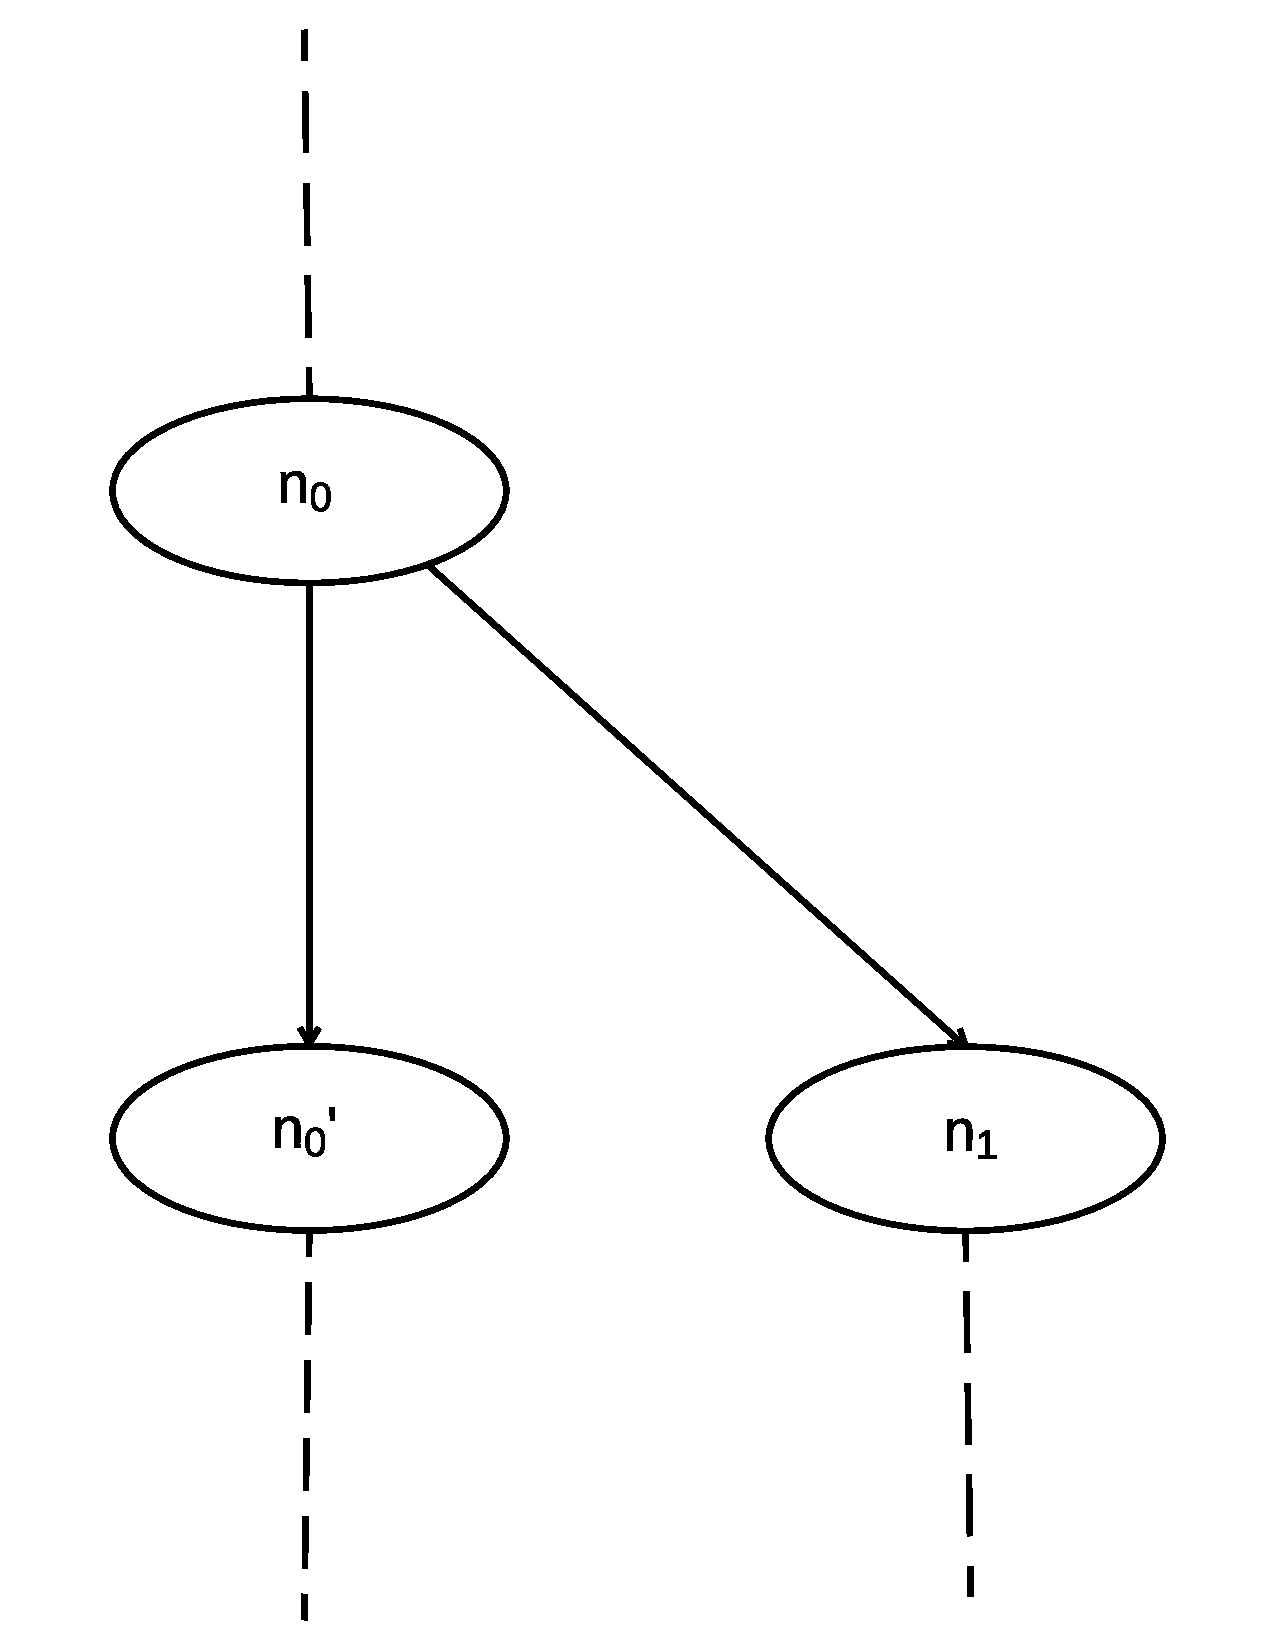
\includegraphics[scale=0.3]{../figs/Fig1-a.pdf}}   
     \subfigure[]{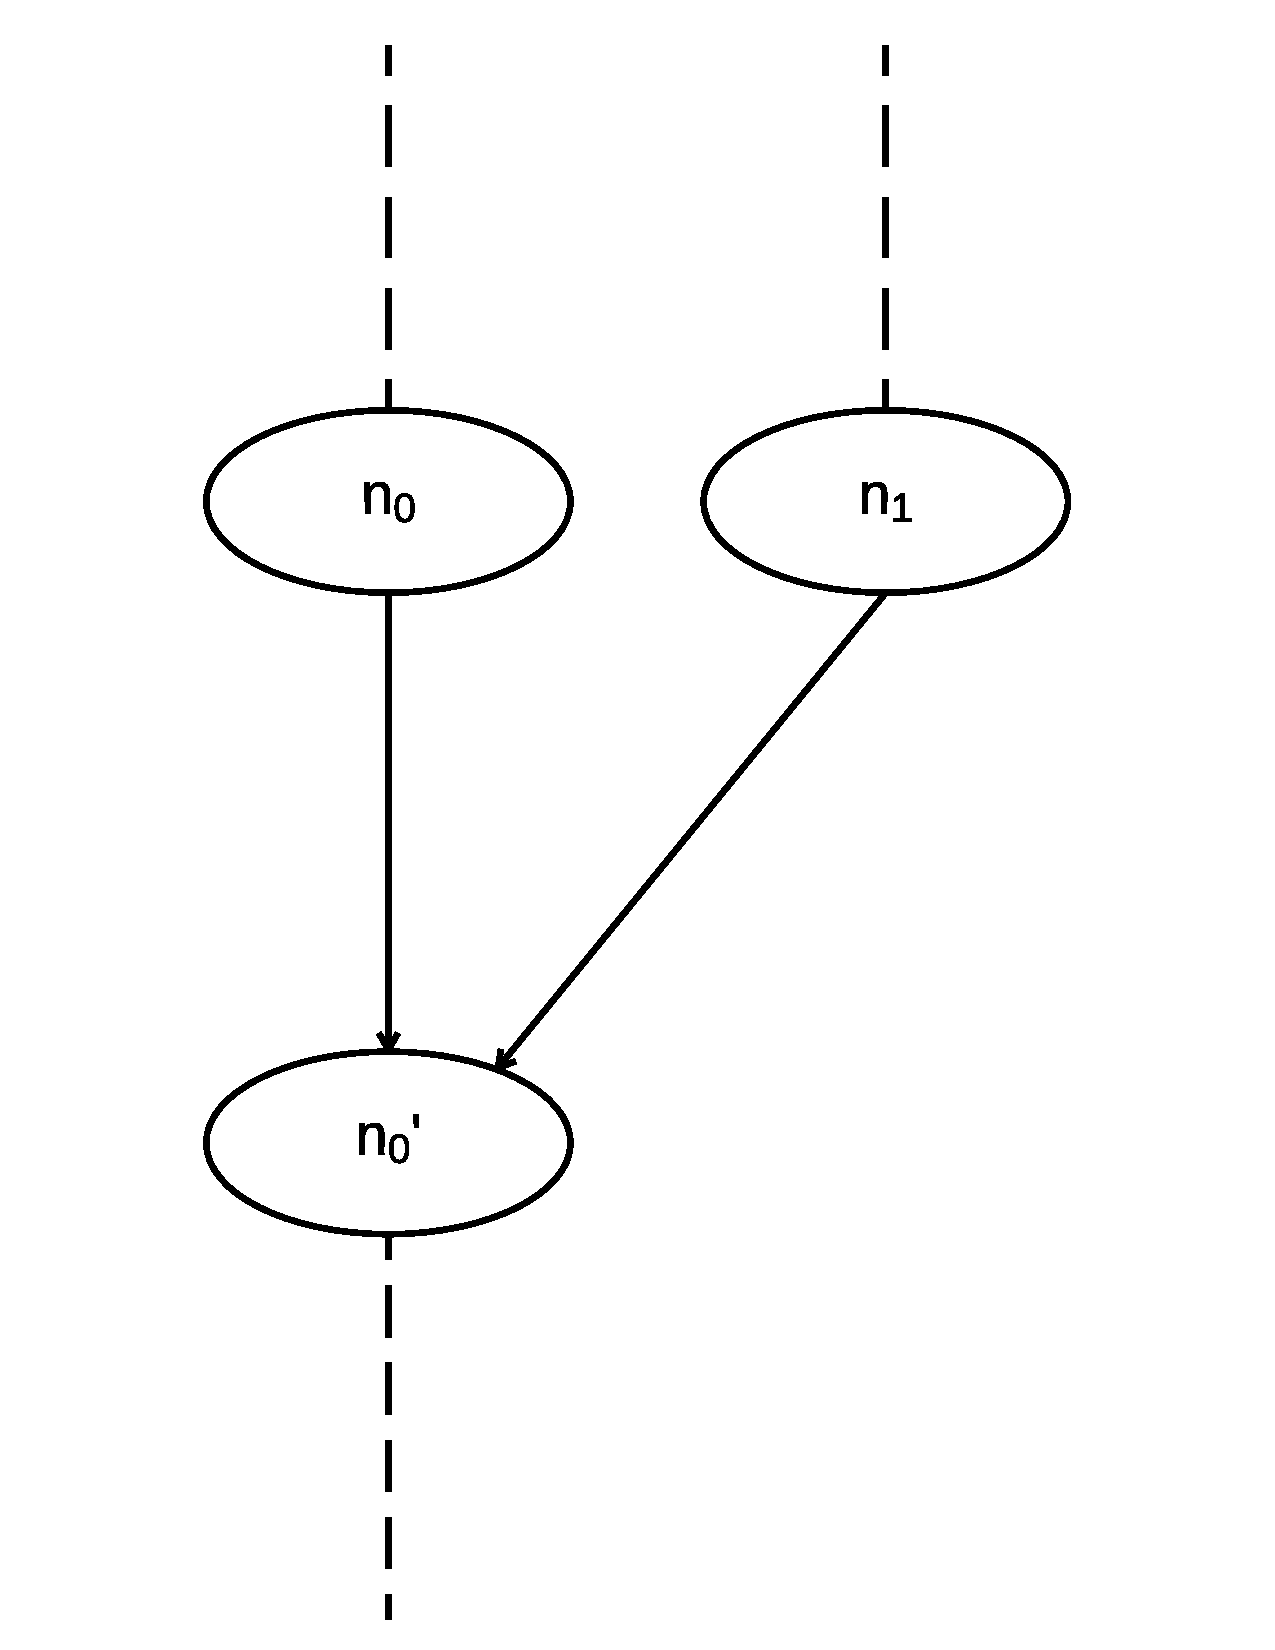
\includegraphics[scale=0.3]{../figs/Fig1-b.pdf}}
  \caption{Steps involved in computation graph creation.}
   \label{fig:cgcreation}
   \end{center}
\end{figure}

The \textsc{Post} rule is fired when the task forks to create a new child task that potentially runs in parallel with the parent task. When a task $t_1$ executes a \textbf{post} statement, two fresh nodes $n_0^\prime$ and $n_1$ are added to the graph. Node $n_0^\prime$ represents the statements following \textbf{post} and $n_1$ represents the statements executed by $t_2$. The current node $n_0$ of $t_1$ is connected to $n_0^\prime$ and $n_1$ as shown in \figref{fig:cgcreation}(a). The read set $\delta$ of node $n_0$ is updated to additionally map to the regions in $\eta(e)$ (i.e., the regions referenced in the expression $e$). The current node of $t_1$ changes to $n_0^\prime$ after the transition. The region mapping $m$ of task $t_1$ is updated by removing the configurations of regions whose ownership is passed to the newly created task $t_2$ and adding a new configuration that consists of the task $t_2$ along with the regions it now owns.

The \textsc{Ewait} rule blocks the execution of the currently executing task until a task in the indicated region completes. The choice of completed task, $t_2$, in the region is non-deterministic. A node $n^\prime$ is added to the graph to act as a join node. It captures the subsequent statements executed by task $t_1$ after the \textbf{ewait} statement finishes. The current node $n$ of task $t_1$ and the current node of task $t_2$, denoted by $n(t_2)$ are connected to $n^\prime$ as shown in \figref{fig:cgcreation}(b). The configuration ($r \mapsto \tuple{t_2,m_2}$) is removed from the region valuation $m$ of task $t_1$. After the transition, the current node of task $t_1$ is changed to $n^\prime$.  The task $t_1$ is resumed with a return value handler for the completed task ($\mathrm{rvh}(t_2)$) before continuing with its next statement.

The \textsc{Await-next} rule blocks the execution of the currently executing task $t_1$ until all the tasks whose handles are stored in region $r$ that the task $t_1$ owns are executed to completion. The rule is implemented recursively by removing one task from the region at a time and then inserting another \textbf{await}-statement on the same region. Similar to \textsc{Ewait}, a join node $n^\prime$ is added to the graph, the current nodes of $t_1$ and $t_2$ are connected to $n^\prime$ as shown in \figref{fig:cgcreation}(b) and the current node of task $t_1$ is changed to $n^\prime$. When task $t_2$ returns a value to $t_1$, $t_1$ executes the statement from the return value handler $\mathrm{rvh}(t_2)$. The \textsc{Await-done} rule terminates recursion when the region is empty. 

The computation graph for the example in \figref{fig:hj-async-finish} is presented in \figref{fig:cg}. When the program starts executing, a node $n_0$ is added to the graph to represent the procedure $main$. When the task $t_1$ is posted by the procedure $main$ to execute procedure $p_1$, two new nodes $n_0^\prime$ and $n_1$ are added to the graph to represent the statements executed by the procedure $main$ and procedure $p_1$ respectively. Similarly, when task $t_2$ is posted by the procedure main to execute procedure $p_2$, two new nodes $n_0^{\prime\prime}$ and $n_2$ are added to the graph. When the main task calls \textbf{await} on $r_1$, its execution is suspended until $t_1$ and $t_2$ finish execution. When the \textbf{await} is executed, node $r_1$ and $r_1^\prime$ are added to the graph. The read and write to region variable $r_1$ by the tasks $t_1$ and $t_2$ is updated in nodes $n_1$ and $n_2$ using the functions $\delta$ and $\omega$ respectively.

The order of synchronization of tasks $t_1$ and $t_2$ affects the value of the variable $n$ in the $main$ task. The return value handlers of the tasks get executed in different orders under different schedules. This makes the output of the program non-deterministic. In a schedule where task $t_1$ joins $main$ task before $t_2$, the value of $n$ at the end of program execution is 3 and in a schedule where task $t_2$ joins $main$ task before $t_1$, the value of $n$ is 2.

\begin{comment}
\begin{theorem}
Algorithm \ref{algo:drd} is complete for a task parallel program with a given input.
\end{theorem}

\begin{proof}
A task parallel program can have different computation graphs based on the schedule followed by the tasks during the program execution. The semantics described in \figref{fig:semantics} show how a computation graph is built for a task parallel program from an observed program execution. The nodes in the graph depict the correct partial order between the tasks in the program. If Algorithm \ref{algo:drd} does not report a race for a computation graph obtained from some execution of the program, data races may still be present under some other program schedule. Therefore, \algoref{algo:drd} is not sound for a task parallel program with a given input. However, if \algoref{algo:drd} reports a data race, then from \thmref{thm:graph} this is a real data race. Therefore, Algorithm \ref{algo:drd} is complete for a task parallel program with a given input.
\end{proof}
\end{comment}

\begin{theorem} \label{thm:cg}
%The computation graph represents the correct partial order relation between the tasks in the program.
The computation graph represents the correct ordering of events in a program and stores the accesses to shared variables in the program. The sequential events are ordered while the concurrent events are unordered.
\end{theorem}

\begin{proof}
Proof by definition: There are two types of operations performed in a task parallel program: inter-procedural and intra-procedural. The inter-procedural statements create different nodes in the graph and are responsible for maintaining the correct ordering of events in the program. The nodes in the computation graph contain read/write sets to store the accesses to shared variables by the tasks. The intra-procedural operations do not affect the structure of the computation graph; however, they update the read/write sets of the nodes in the computation graph when the tasks access shared variables. These operations are discussed separately below.
 
The semantics for inter-procedural statements are given in \figref{fig:semantics}.
The inter-procedural statements are \textbf{post}, \textbf{ewait}, \textbf{await} and \textbf{call}. When a \textbf{post} statement is executed, the \textsc{Post} rule is fired. It creates two new nodes in the computation graph. One node represents the statements executed by the newly posted task and the other node represents the statements executed by the calling task immediately following the \textbf{post} statement. These nodes are set as the active nodes for these tasks. Any access to the shared memory is stored in the read/write sets for the active node. These two nodes are unordered since the statements are executed concurrently by these tasks.

 The \textbf{ewait} is used to synchronize a child task with its parent task. The \textsc{Ewait} rule creates a join node in the computation graph. Both the child and the parent task's active nodes are connected to the join node. The added edges order this node after the active nodes in the child task and the parent task. The \textbf{await} statement joins all the children tasks posted in a region to the parent task. The \textbf{await} statement fires the \textsc{Await-next} rule that joins one child task at a time to the parent task. Similar to the \textsc{Ewait} rule, \textsc{Await-next} also creates a join node for every child task. The join node is set as the active node for the calling task. Any shared memory accesses by the calling task are registered in the read/write sets of the active node.
 
Finally, the \textbf{call} is semantic sugar for a \textbf{post} followed by an \textbf{ewait}. As such, even though the calling task gets a new active node to reflect its concurrent relationship to the newly created task, the read/write sets in that node are never updated since the calling task executes \textbf{ewait} immediately after the \textbf{post}, which does not read/write any region variables, and once the \textbf{ewait} completes, the task gets a new active node ordered after the join from the task created by the call.

The intra-procedural statements are \textbf{assign}, \textbf{skip}, \textbf{assume}, \textbf{if-then-else} and \textbf{do-while}. The semantics for intra-procedural statements is given in \figref{fig:intra}. The semantic rules for intra-procedural events show that they do not change the structure of the computation graph since none of the rules create any new nodes or edges in the computation graph.

The \textsc{Skip} rules does not interact with any shared variables in the program. The \textbf{if-then-else} and \textbf{do-while} statements fire \textsc{If-then}, \textsc{If-else}, \textsc{Do-loop} and \textsc{Do-break} rules. These rules only read shared variables. Therefore, only the read sets for the active nodes set by the inter-procedural statements are updated by the statements. The \textsc{Assign Local} rule only updates the read set of the active node since this rule does not update any shared variables. Whereas the \textsc{Assign Region} rule updates both read/write sets of the active node, since shared program variables are updated by this rule. As such, by definition, the computation graph exactly reflects the orders defined by the semantics and only updates read/write sets that are defined by the semantics.
\end{proof}

\begin{corollary}
%\algoref{algo:drd} is complete for a task parallel program with a given input.
Applying \algoref{algo:drd} to computation graphs created using the semantics of task parallel programs is complete for data race detection in the given program input -- data race free programs will never be rejected; but, programs with data race may be accepted because the data race did not manifest in the computation graph from the executed schedule.
\end{corollary}

\begin{proof}
Proof by example: A task parallel program can have different computation graphs based on the schedule followed by the tasks during the program execution. If \algoref{algo:drd} does not report a race for a computation graph obtained from some execution of the program, data races may still be present under some other program schedule. 

\begin{figure}
  \begin{center}
    \begin{lstlisting}[mathescape=true]
  proc main(var n : int)
  	n := 1;
  	post $r_1 \leftarrow p_1~n~\varepsilon~\{r_1\}~\{r_1\}~\lambda v. n := v$;
  	post $r_1 \leftarrow p_2~n~\varepsilon~\{r_1\}~\{r_1\}~\lambda v. n := v$;
  	ewait $r_1$ 
  	if $(n == 1)$ then
      post $r_1 \leftarrow p_3~n~\varepsilon~\{r_1\}~\{r_1\}~\lambda v. n$;
      $r_1 := 1$
   await $r_1$
 proc $p_1$(var n : int)
 	return 0
 proc $p_2$(var n : int)
	return 1
 proc $p_3$(var n : int)
	$r_1 := 2$
\end{lstlisting}
  \end{center}
  \caption{Parallel program with different computation graphs under different schedules.}
  \label{fig:diffCGs}
\end{figure}

\begin{figure}
  \centering
  \subfigure[$t_1$ joins first.]{\includegraphics[scale=0.35]{../figs/Figa.pdf}}
  \subfigure[$t_2$ joins first.]{\includegraphics[scale=0.35]{../figs/Figb.pdf}}
  \caption{Computation graphs of example in \figref{fig:hj-isolated}.}
   \label{fig:diffCGsfig}
\end{figure}

Consider the example in \figref{fig:diffCGs}. The task parallel program in the example has a data race under one program schedule and it is data race free under a different schedule. The computation graphs for the different schedules are shown in \figref{fig:diffCGsfig}. If the program follows the first schedule, (i.e., task $t_1$ joins before $t_2$) task $t_3$ is not spawned and there is no data race in the program. If the program, however, follows the second schedule(i.e., task $t_2$ joins first), then a new task $t_3$ is created by task $t_0$ and there is a data race on region variable $r_1$. 
%This example shows that \algoref{algo:drd} is not sound for task parallel programs with a given input. 

\thmref{thm:graph} shows that \algoref{algo:drd} is sound and complete for a given computation graph. When \algoref{algo:drd} is applied to task parallel programs with a given input, it may accept programs as data race free that in reality contain data races. This is evident from example in \figref{fig:diffCGs}. Therefore, determining data race freedom from a single schedule of a task parallel program using \algoref{algo:drd} is complete for the input program because different schedules create different computation graphs. 

%From \thmref{thm:cg}, it can be seen that a computation graph represents the correct partial order relation between the tasks of the program. \thmref{thm:graph} shows that a data race reported in the computation graph for the given program schedule is guaranteed to be a real data race. Therefore, \algoref{algo:drd} is complete for a task parallel program with a given input.
\end{proof}